\begin{pastexam}[label={px:ntu-112-dsa-02}]{臺大資工所 112 學年度 第 2 題}
（複選；5 分，每個選項單獨計分，答對得 1 分、答錯倒扣 0.5 分）

B+ tree is an extension of B tree. The major differences from B tree are (1) all leaf nodes are
linked together in a doubly-linked list, and (2) data points are stored on the leaf nodes only;
internal nodes only hold keys and act as routers to the correct leaf node; the left child is
smaller than the key and the right child is larger or equal than that. Please find any/all
\underline{violations} of a B+ tree structure in the following diagram. Assume the tree node can at
most contain 4 data points (keys).

\begin{center}
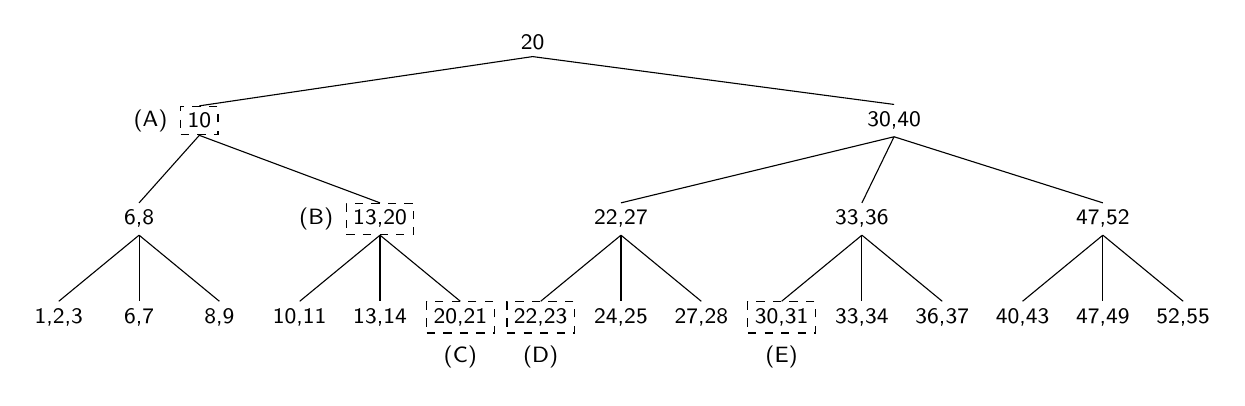
\begin{tikzpicture}[x=1.02cm,y=1cm,font=\sffamily\footnotesize,k/.style={inner sep=2.5pt},v/.style={k,draw,dashed}]
\node[k] (l0) at (0,0) {1,2,3};
\node[k] (l1) at (1,0) {6,7};
\node[k] (l2) at (2,0) {8,9};
\node[k] (l3) at (3,0) {10,11};
\node[k] (l4) at (4,0) {13,14};
\node[v] (l5) at (5,0) {20,21};
\node[v] (l6) at (6,0) {22,23};
\node[k] (l7) at (7,0) {24,25};
\node[k] (l8) at (8,0) {27,28};
\node[v] (l9) at (9,0) {30,31};
\node[k] (l10) at (10,0) {33,34};
\node[k] (l11) at (11,0) {36,37};
\node[k] (l12) at (12,0) {40,43};
\node[k] (l13) at (13,0) {47,49};
\node[k] (l14) at (14,0) {52,55};
\node[k] (m0) at (1,1.25) {6,8};
\node[v] (m1) at (4,1.25) {13,20};
\node[k] (m2) at (7,1.25) {22,27};
\node[k] (m3) at (10,1.25) {33,36};
\node[k] (m4) at (13,1.25) {47,52};
\node[v] (a) at (1.75,2.5) {10};
\node[k] (b) at (10.4,2.5) {30,40};
\node[k] (r) at (5.9,3.5) {20};
\node[left=1pt] at (a.west) {(A)};
\node[left=1pt] at (m1.west) {(B)};
\node[below=1pt] at (l5.south) {(C)};
\node[below=1pt] at (l6.south) {(D)};
\node[below=1pt] at (l9.south) {(E)};
\draw (r.south)--(a.north) (r.south)--(b.north);
\draw (a.south)--(m0.north) (a.south)--(m1.north);
\draw (b.south)--(m2.north) (b.south)--(m3.north) (b.south)--(m4.north);
\draw (m0.south)--(l0.north);
\draw (m0.south)--(l1.north);
\draw (m0.south)--(l2.north);
\draw (m1.south)--(l3.north);
\draw (m1.south)--(l4.north);
\draw (m1.south)--(l5.north);
\draw (m2.south)--(l6.north);
\draw (m2.south)--(l7.north);
\draw (m2.south)--(l8.north);
\draw (m3.south)--(l9.north);
\draw (m3.south)--(l10.north);
\draw (m3.south)--(l11.north);
\draw (m4.south)--(l12.north);
\draw (m4.south)--(l13.north);
\draw (m4.south)--(l14.north);
\end{tikzpicture}
\end{center}
\end{pastexam}

\begin{pastsoln}
答案：(A)、(B)、(C)、(D)。

先把題目的規則講清楚。 每個節點最多 $4$ 個鍵，所以內部節點最多 $5$ 個子節點，也就是 $m = 5$ 階。
B$^{+}$ 樹的內部節點規則和 B 樹一樣（資結書第~11.2~節、第~11.3~節）：根以外的內部節點至少
$\lceil m/2 \rceil = 3$ 個子節點、至少 $2$ 個鍵；葉子至少半滿，也就是至少 $2$ 筆資料。 分隔鍵的規則照
題目：左邊子樹的鍵都 $<$ 分隔鍵，右邊子樹的鍵都 $\ge$ 分隔鍵。 這個規則要從根一路往下累積：
一個節點的鍵，必須落在祖先的分隔鍵給它的範圍裡。

由根往下標出每個節點應該在的範圍，再一一檢查：
\begin{center}
\small
\begin{tabular}{ll>{\raggedright\arraybackslash}p{0.5\linewidth}}
\toprule
節點 & 應該在的範圍 & 檢查 \\
\midrule
根 $20$ & 全部 & 根可以只有 $1$ 個鍵 \\
(A) $10$ & $< 20$ & 鍵本身沒問題，但只有 $1$ 個鍵、$2$ 個子節點，\textbf{不滿 $3$ 個子節點} \\
$6, 8$ & $< 10$ & 對；三片葉子 $\{1,2,3\}$、$\{6,7\}$、$\{8,9\}$ 也都在範圍裡 \\
(B) $13, 20$ & $[10, 20)$ & \textbf{$20$ 不在 $[10, 20)$ 裡} \\
葉子 $10,11$、$13,14$ & $[10, 13)$、$[13, 20)$ & 對 \\
(C) 葉子 $20, 21$ & $[20, 20)$，空的 & \textbf{$20, 21 \ge 20$，應該在根的右邊} \\
$30, 40$ & $\ge 20$ & 對 \\
$22, 27$ & $[20, 30)$ & 對 \\
(D) 葉子 $22, 23$ & $[20, 22)$ & \textbf{$22, 23 \ge 22$，應該在 $22$ 的右邊} \\
葉子 $24,25$、$27,28$ & $[22, 27)$、$[27, 30)$ & 對 \\
$33, 36$ & $[30, 40)$ & 對 \\
(E) 葉子 $30, 31$ & $[30, 33)$ & 對 \\
其餘葉子 & & 都在各自的範圍裡 \\
\bottomrule
\end{tabular}
\end{center}

逐項看：
\begin{itemize}
\item \textbf{(A) 違規。} 它的鍵和子樹都沒放錯（左邊 $1$--$9$ 都 $< 10$），問題在大小：$5$ 階的
B$^{+}$ 樹，根以外的內部節點至少要 $3$ 個子節點，這個節點只有 $2$ 個。 其他內部節點都有 $2$ 個鍵、
$3$ 個子節點，只有它不夠。
\item \textbf{(B) 違規。} 它在根的左子樹裡，裡面的鍵都必須 $< 20$，分隔鍵 $20$ 卻不是。
\item \textbf{(C) 違規。} $20, 21$ 都 $\ge$ 根的分隔鍵 $20$，照規則要走右子樹，卻放在左子樹；照這
棵樹搜尋 $20$ 會往右走，找不到它。
\item \textbf{(D) 違規。} 它是 $22, 27$ 最左邊的子節點，裡面的鍵必須 $< 22$，但 $22, 23$ 都不是；
搜尋 $22$ 會走到中間那片 $24, 25$，找不到。
\item \textbf{(E) 沒有違規。} 它的範圍是 $[30, 33)$（根的右邊 $\ge 20$、$30, 40$ 的中間 $[30, 40)$、
$33, 36$ 的最左邊 $< 33$），$30, 31$ 都在裡面，大小也有 $2$ 筆。
\end{itemize}
附帶一提，從左到右的葉子 $1, 2, 3, 6, \ldots, 55$ 本身是由小到大的，(B)(C)(D) 錯的是分隔鍵和葉子的
對應，不是葉子的順序。
\end{pastsoln}
